This section will first discuss the forms of organizational structure defined in the literature. Second, the (de)centralization of current organization and, as a consequence, their styles of IT governance will be explored. We conclude this section by underpinning the challenges organizations have to face due to their progressive decentralization.

\subsection{What is a Decentralized Organization?} 
 
An organization can be structured in many different ways. Sachdeva \cite{sachdeva1990} defines organizational structure as "... institutional arrangements and mechanisms for mobilizing human, physical, financial and information resources at all levels of the system..." According to Jacobides \cite{jacobides2007}, "Organizational structure provides the frames through which individuals see their world. Thus, the way each organization is structured shapes an ecology of different, distinct frames that exist at the level of the organizational subunit." 
%Nystrom and Starbuck \cite{nystrom1981} define organisational structure as the arrangement and interrelationship of component parts and positions in an organization.

There has been a lot of research on specific forms of organizational structure. Taxonomies of organization forms are defined in  \cite{mckelvey1982}, \cite{rich1992}.   \textit{Classic} and \textit{modern} types of organizational structure are often recognized.  Classic types include simple centralized organizations ~\cite{Mintzberg1979}, bureaucratic organizations \cite{mintzberg1981}, divisional structure and functional structure. Modern  types include matrix structure, flat organizations, adhocracy. New forms of organizational structure emerged recently: collaborative networks, virtual organizations and coopetition.

According to Robbins \cite{robbins1997}, organizational structure has three components: complexity, formalization and centralization.  Complexity refers to the degree to which activities within the organization are differentiated; Formalization refers to the degree to which work is standardized; Centralization refers to the degree to which decision making is concentrated at one point in the organization. 

Following Luthens \cite{luthans2006}, centralization and decentralization can be also defined according to three factors: geographical or territorial concentration or dispersion of operations; functions;  extent of concentration or delegation of decision making powers. In \cite{pearlson2009},  the following characteristics of centralization are defined: the allocation of decision rights,  the structure of communication lines and  the choice of forms of coordination.

In a centralized organization, all decision making authority would reside with a single, top-level authority. In a completely decentralized enterprise all members would have equal decision making rights. Here, hierarchy manages the inter-dependencies between the different subunits of organization and often makes direct interactions and communications unnecessary \cite{thompson1967}.  Decentralized organizations instead have less formalized communication lines~\cite{pearlson2009, ahuja1998network}, and more fluid, project oriented teams.~\cite{applegate1988}

Centralized organizations lean towards primarily vertical style of coordination~\cite{Bolman2008}, which is characterized by formal authority, standardization and rules in operations and in IT, and planning and control systems. Decentralized organizations lean towards lateral coordination characterized by meetings, task forces, coordinating roles, matrix structures, and networks~~\cite{Bolman2008}. 

Below, popular forms of organizations focusing on their degree of centralization will be considered. 

\subsection{Forms of Organizational Structure and Decentralization}

\subsubsection{Classic Organizational Structures}

Pearlson and Saunders offer a thorough description of a pure hierarchical organization structure~\cite{pearlson2009}: Except for the top level position, each position has one superior and zero or more subordinates. Decision rights and communication lines are strictly defined and work their way down from the top (i.e. the center). The scope of a position is specialized and strictly defined by your superior and one works in assigned teams. The primary benefit of a hierarchy is that the high levels of management have strict governance and control over the company. Hierarchical organization structures are suited for stable, certain environments. 

Hierarchical organizations can be subdivided into simple centralized and bureaucratic organizations:

In simple centralized organizations, both strategic planning and operational decision making authority belongs to one person at the top. This structure can be found in small and single-person-owned organizations with only two hierarchical levels. 

Bureaucratic organizations \cite{mintzberg1981} are characterized by multi-level hierarchical structure and use of standard methods and procedures for performing work. 

Hierarchical organizations generally divide their labor either in terms of function, a grouping of common activities, or in terms of division, a grouping based on output (product). Two organizational structures, divisional and functional, can be identified accordingly.

\subsubsection{Modern Organizational Structures}

Matrix structure is another popular style of organization structure~\cite{pearlson2009} that can be seen as a mixture of functional and divisional structures. In this form, individuals are assigned two or more supervisors covering different (usually product and functional) dimensions of the enterprise. Pearlson and Saunders state that matrix organization structures are suited for dynamic environments with lots of uncertainty, presumably because their authority structure allows them to cover multiple aspects when making decisions. However, like a hierarchical structure, a matrix structure is a rigid construct with strictly defined roles, communication lines and decision rights. Authority still comes from the top in a centralized manner, even though it becomes more distributed among matrix managers at the lower levels~\cite{pearlson2009}. 
%Consequently, matrix structures still may not be perfectly suited for uncertain, dynamic environments. 

%Applegate, Cash, and Mills~\cite{applegate1988} support this statement, as they describe hierarchical and matrix structures as rigidly structuring "communication, responsibility, and accountability to help reduce complexity and provide  stability". They furthermore state that both matrix and hierarchical structures have the effect of stifling creativity and preventing organizations from being able to adapt effectively to rapidly changing environments. 

Flat organization is a novel type of organizations where only one or maximum two hierarchical levels are defined (similarly to simple centralized organizations). For example, Valve Corporation, a software company in the video game industry released their handbook in 2012~\cite{valveHandbook}.  Unlike simple centralized organization described above, individual employees have complete freedom despite there being a president/founder at the top: Nobody reports to anyone, and everyone is free to work on whatever they want to. This is an example of high decentralization.

Adhocracy~\cite{applegate1988,pearlson2009}  aims to discard traditional hierarchies in favor of decentralized decision rights and flexible communication lines connecting the entire enterprise. Specifically, instead of hierarchies, an adhocracy has a rapidly changing set of project oriented groups that have decision making authority and other powers  \cite{robbins1997}. Mintzberg describes an adhocracy as "a loose, flexible, self-renewing organic form tied together mostly through lateral means"~\cite{Mintzberg1979}.  

\subsubsection{Post-Modern Organizational Structures}

New forms of organizational structure enabled uniquely by modern information and communication technologies  Internet emerged recently:  collaborative networks~\cite{Camarinha-Matos2005} and coopetitions~\cite{Bengtsson2000}.

%Network organizations are characterized by subcontracting  their business functions \cite{????};

Related to the idea of adhocracy, is the concept of collaborative networks (CN). Camarinha-Matos and Afsarmanesh define collaborative networks as being composed of ``a variety of entities (e.g., organizations and people) that are largely autonomous, geographically distributed, and heterogeneous in terms of their: operating environment, culture, social capital, and goals.''~\cite{Camarinha-Matos2005} Three common characteristics in various CNs are autonomy in the individual entities, a drive towards meeting common or complementing goals, and the use of an agreed-upon framework for collaboration. 

Under the umbrella of CNs, Camarinha-Matos and Afsarmanesh define virtual organizations, virtual communities, and virtual breeding environments~\cite{Camarinha-Matos2005}. Virtual organizations are a group of independent organizations working together to achieve some goal(s); virtual communities are communities of individuals that interact with each other through the use of computer network-based technologies; and virtual breeding environments are frameworks for interoperability set up by groups of organizations in order to enable the potential for forming a virtual organization.

%These entities collaborate through  computer networks in order to achieve common or complementary goals. The main driver behind CNs is that the goals the seek to achieve would be impossible or much more difficult to achieve without collaboration. %The composition of autonomous entities makes CNs a very relevant concept to decentralization. 

Another organizational form emerged recently is coopetition. Bengsston and Kock describe coopetition as a complex relationship between firms where they simultaneously compete and collaborate and benefit from both~\cite{Bengtsson2000}. Coopetition allows the participating organizations to take advantage of a heterogeneity of resources. Organizations may seek to create competitive advantage through a unique resource they own (e.g. skill). At the same time, it might be beneficial for them to cooperate with another organization that possesses a unique resource that is of value to them. 

Virtual organizations and coopetitions differ from the organizational structures defined above since they do not represent a single legal entity but a group of autonomous and independent entities with different (and possibly concurrent) strategic goals. These entities are engaged into collaboration in response to factors such as specific market situations, customer demand, etc.  The heterogeneous structure of such organizations remains invisible for a customer, while the service level agreements should be maintained at the same high level any other organization would maintain. Such organizational structures are grounded on a sustainable collaboration between partners without any centralized control.

%They explore the concept of coopetition in the context of competing firms that "produce and market the same product".~\cite{Bengtsson2000} In this context, they place an important limit on coopetition: their needs to be some kind of separation between the competing and cooperating aspects i.e. they can not "coopetate" in the same aspect. 

%An example of coopetition is Amazon.com's Marketplace; a platform provided by Amazon where any  competitor can list items for sale alongside Amazon's own sales, often of the same items~\cite{UnknownAskIrina,Amazon.com}. This allows sellers to take advantage of Amazon's platform while Amazon takes advantage of the increase in traffic. 

\subsubsection{Decentralization in Organizational IT}
According to Rockart et al.\cite{Rockart1996}, changes in business and technology as well as progressive decentralization of organization as a whole drives the changes in roles and structure  of IT units. The works presented in \cite{fulk1995, osterloh2000, Rockart1996, Weill2004} focus on the relation between the structure of an organization and its IT. 

Fulk \cite{fulk1995} discusses the interplay between communication technology and various organizational forms. The authors consider communication technologies as one of the key enablers of inter-organizational and intra-organizational changes.

In \cite{osterloh2000}, authors study how different organizational forms affect the knowledge transfer in organization. They claim that ``Organizational forms enable different kinds of motivation and have different capacities to generate and transfer tacit knowledge.''

Weill~\cite{Weill2004} defines six forms of organizational structures in IT (called IT Governance archetypes) based on how the five major IT decisions in organizations are made. These archetypes are: business monarchy, IT monarchy, feudal, federal, IT duopoly and anarchy.   In a \textit{business monarchy} all IT related decisions are made in a centralized manner by the top-level executives (e.g. the CxOs). In an \textit{IT monarchy}, a group of IT professionals are responsible for making the decisions. This is also highly centralized as the authority resides with this group. An \textit{IT duopoly} is characterized by two groups, one of IT executives and the other of business executives, coming to agreements in order to make decisions. This is more centralized than the federal form, as the decisions are only made by the two groups, rather than each individual business unit having input. The \textit{feudal} is much less centralized. It is where individual organizational units are responsible for their own decisions. \textit{Federal IT  }would aim to balance these through a combination of central IT and IT in the business units. \textit{Anarchy} is a highly decentralized style of governance. It is similar to the feudal archetype, however the size of the units is much smaller. Instead of being an entire business unit, small teams or even individuals are responsible for their own decisions.

%This allows for systems that meet the individual business units needs, as well as enabling interoperability throughout the enterprise. 



%\subsection{IT Governance}

%\cite{Rockart1996} Some key weaknesses of centralized IT to eliminate are slow responsiveness and having systems that do not fit the needs of individual business units. Decentralized IT on the other hand lacks "synergy and integration"~\cite{Rockart1996} due to a lack of standardization.

% CAN GO TO THE SOLUTION PART? Federal IT would aim to balance these through a combination of central IT and IT in the business units. A primary task of the central IT would be to maintain standards for the entire enterprise. The business units would still have ownership of many of their own systems, allowing them to implement them as they deem best. This allows for systems that meet the individual business units needs, as well as enabling interoperability throughout the enterprise. 
%
%
%\begin{figure}
%\centering
%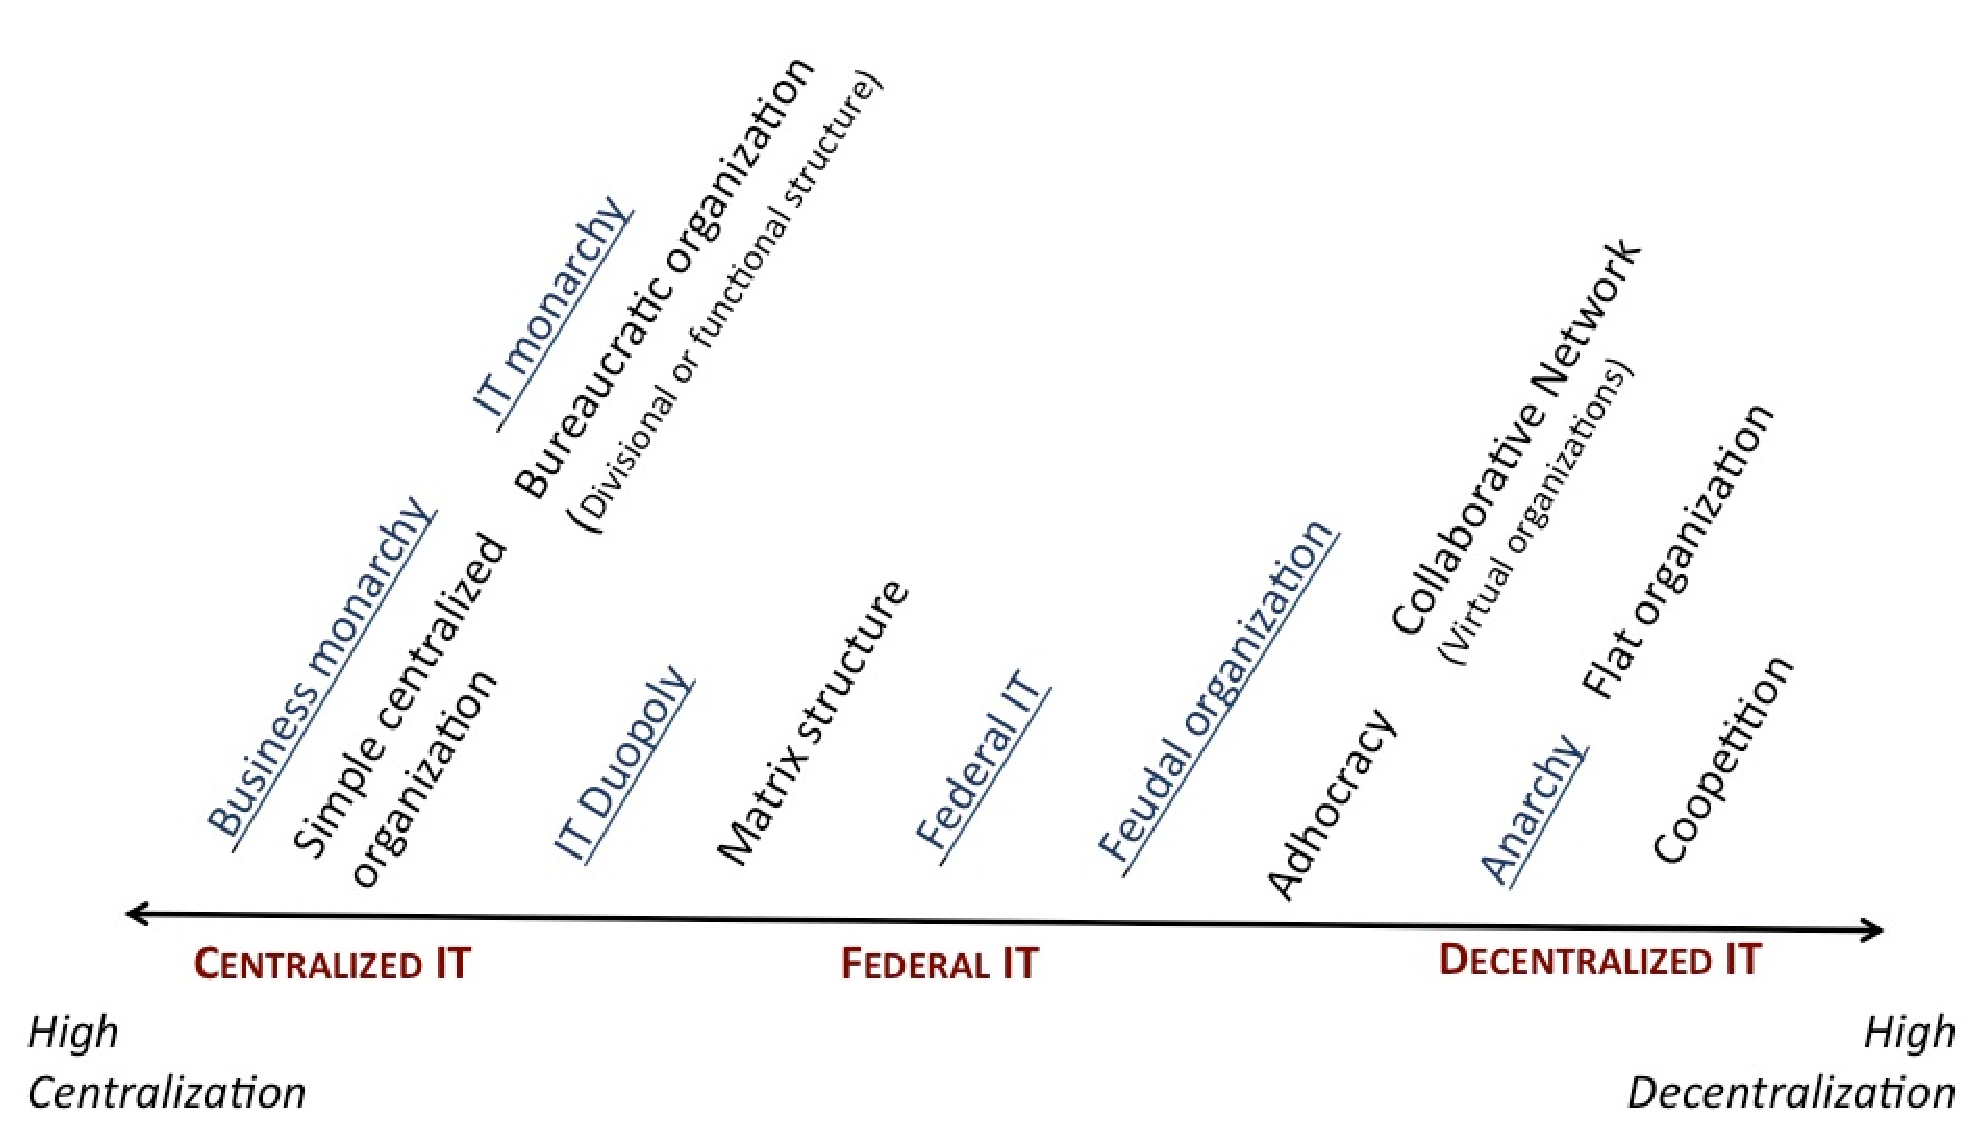
\includegraphics[scale=0.3]{taxonomy}
%\caption{Organizational taxonomy: From Centralized to Decentralized}
%\label{fig:taxonomy}
%\end{figure}

\subsection{Challenges of Progressive Decentralization in Organizational IT}
\label{sec:challenge}

%The trend appears to be moving away from the paradigm within which organizations strive for mass production efficiencies, hierarchical organization, and bureaucratic structures that provide central control over activities divided into small parts. The new paradigms may have as their premise the needed for flexible, learning organizations that continuously change and solve problems through interconnected coordinated self-organizing processes.

%From: Daft, Richard L., and Arie Y. Lewin. "Where are the theories for the" new" organizational forms? An editorial essay." Organization Science 4.4 (1993): i-vi.

%********

Modern organizational structures show a strong tendency towards decentralization \cite{daft1993} which results in changes to their management and operation styles. This heavily involves IT and requires major changes in organization processes. This transformation is not a mere question of ``flattening'' the organization by shifting authorities and decision making power from top to bottom hierarchical levels or from one person to a group. In classic organizations, not only does hierarchy ensure control and coordination, it also manages interdependencies between  different subunits of an organization which often makes direct interaction and communication unnecessary \cite{thompson1967}. As a result, a challenge related to decentralization and a ``weakened hierarchy'' is a lack of interaction and communication between organizational subunits. Another major risk of IT decentralization, according to \cite{Rockart1996}, is poor synergy and integration due to a lack of standardization.

Caruso, Rogers and Bazerman~\cite{caruso2008boundaries} highlight the importance of information sharing and coordination for these organizations. In order to succeed at these aspects, they outline three barriers that decentralized organizations need to overcome. The first barrier is intergroup bias; the tendency to treat one's own group better than other groups. The second barrier is group territoriality; the tendency for a group to protect their territory (physical or informational). The third barrier is poor negotiation strategies used by different groups when interacting with one another. 

Intergroup bias is direct result of having separate, autonomous groups within an enterprise~\cite{caruso2008boundaries}. The individual groups have a tendency to promote their own group over other groups, especially in situations where they are competing for a resource, such as a portion of the budget. A certain level of competition can be beneficial, however if it leads to hostility or distrust between groups, this can have a detrimental effect on their ability to share information and collaborate. This can prevent the groups from taking advantage of situations where they have to ability to work together for the benefit of everyone. 

The second barrier identified by Caruso et al. is group territoriality~\cite{caruso2008boundaries}. Group territoriality is characterized by group members taking action in order to protect their perceived territory. This can include physical territory such as space or tangible resources, as well as intangible territory, such as roles or information. Group territoriality is supported by a group's need to maintain its identity, its reputation of competence and sense of value, and a group's need for a stable home within the organization from which they interact with the rest of it. Group territoriality encourages ``a sense of psychological ownership''~\cite{caruso2008boundaries} for a group's members which can enforce the belief that they are the sole responsible party for a role or specific knowledge. This "inward-looking" behavior works against collaboration and information sharing. On the other hand, group territoriality can be beneficial; it can foster a sense of security in its members that ``facilitates planning and execution of activities''~\cite{caruso2008boundaries}. 

The third barrier identified by Caruso et al. in decentralized organizations is related to negotiations between groups, and how these negotiations are often conducted using ``poor negotiation  strategies''~\cite{caruso2008boundaries}. These poor strategies are the result of three common errors made while negotiating. The first error is a false belief in a ``fixed pie'' of value that is to be divided when negotiating. This prevents negotiating parties from recognizing situations where they are able to help each other, and therefore increase the size of the figurative pie. The second error is a failure to properly consider the other group's perspective. Understanding the other group's decision process, valuing process, and interests is key to discovering opportunities for helping one another, and the organization as a whole. The third error is when groups fail to even recognize they are in the process of negotiating. Instead, they see it as a competitive or hostile behavior where, again, they only see a fixed pie that is to be split up. This also prevents groups from taking advantage of opportunities to increase the size of the pie.    



